% Section content template for individual Educative lessons
% This file contains the actual content for a specific section
% Generated from Educative API section content

% Section: System Design: The Distributed Task Scheduler
% Section ID: 6152021643624448
% Section Slug: system-design-the-distributed-task-scheduler
% Generated: 2025-12-07T22:08:54.079545

\subsection{What is a task scheduler?}\label{zjrhHwmiCkLLclgfHxbnd}
\\
A \textbf{task} is a piece of computational work that requires resources (CPU time, memory, storage, network bandwidth, and so on) for some specified time. For example, uploading a photo or a video on Facebook or Instagram consists of the following background tasks:

\begin{figure}[htbp]
 \centering
 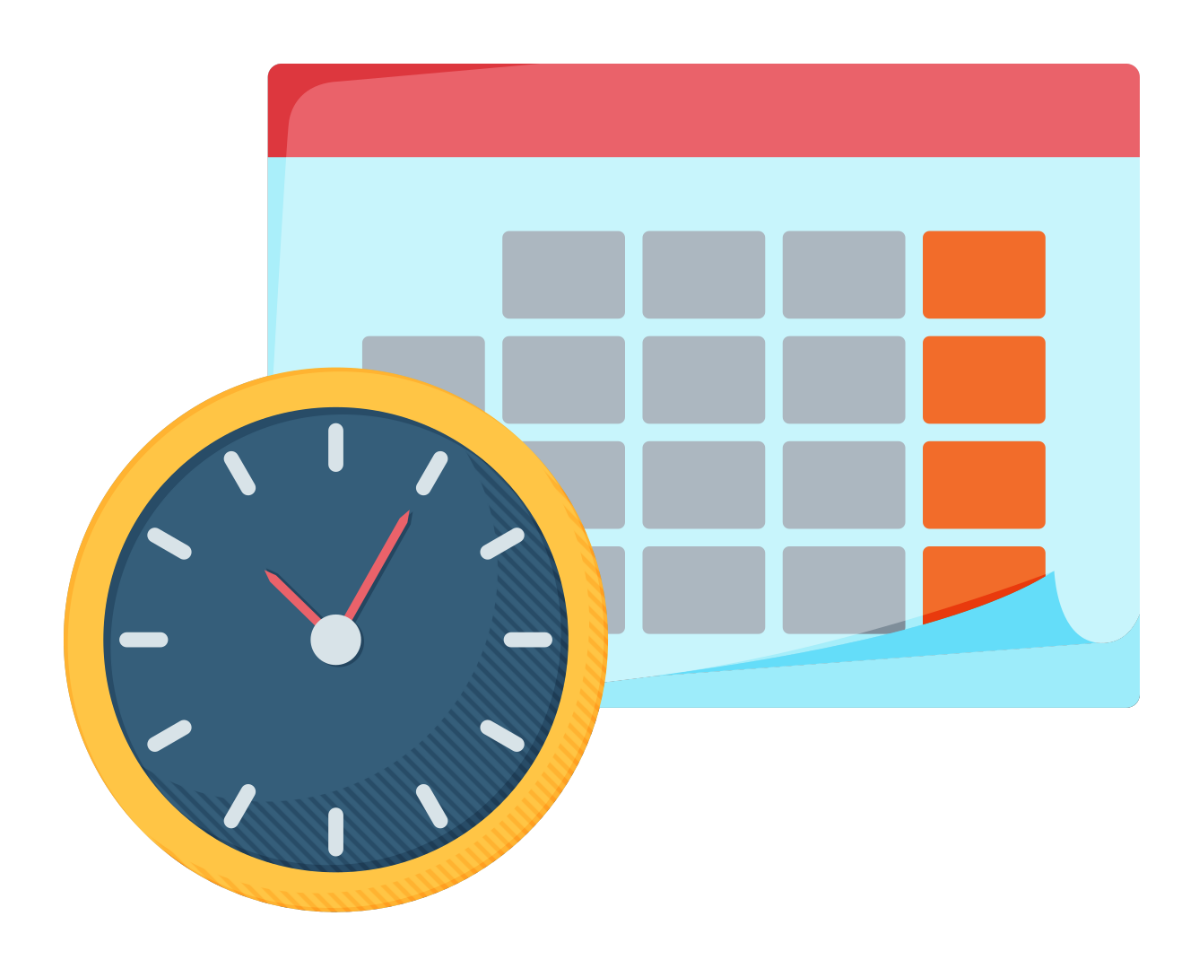
\includegraphics[width=0.15\textwidth]{Images/chapter_23/section_6152021643624448/5944815097085952.png}
 
\end{figure}

\begin{enumerate}
\item
\protect\phantomsection\label{--i2wlTvQiD1Pk2qqkNFP}
Encode the photo or video in multiple resolutions.
\item
\protect\phantomsection\label{XQFc9tKUCAylRcrl4z7pV}
Validate the photo or video to check for content monetization(Content monetization is a way of leveraging content so that a service can profit from it as users consume it.) copyrights, and many more.
\end{enumerate}
\\
The successful execution of all the above tasks makes the photo or video visible. However, a photo and video uploader does not need to stop the above tasks to complete.
\\
Another example is when we post a comment on Facebook. We don't hold the comment poster until that comment is delivered to all the followers. That delivery is delegated to an asynchronous task scheduler to do offline.
\\
In a system, many tasks contend for limited computational resources. A system that mediates between tasks and resources by intelligently allocating resources to tasks so that task-level and system-level goals are met is called a \textbf{task scheduler}.

\subsection{When to use a task scheduler}\label{B4RR4tT_obabcovGm18Nc}
\\
A task scheduler is a critical component of a system for getting work done efficiently. It allows us to complete a large number of tasks using limited resources. It also aids in fully utilizing the system's resources, provides users with an uninterrupted execution experience(Running periodic tasks without user intervention to initiate the task execution again and again.), and so on. The following are some of the use cases of task scheduling:

\begin{itemize}
\item
\protect\phantomsection\label{kcxYpOO9hEzD2wxQnmlcH}
\textbf{Single-OS-based node:} It has many processes or tasks that contend for the node's limited computational resources. So, we could use a local OS task scheduler that efficiently allocates resources to the tasks. It uses multi-feedback queues to pick some tasks and runs them on some processor.
\item
\protect\phantomsection\label{wfsyejuy65KKZ0j71bmhX}
\textbf{Cloud computing services:} Where there are many distributed resources and various tasks from multiple tenants, there is a strong need for a task scheduler to utilize cloud computing resources efficiently and meet tenants' demands. A local OS task scheduler isn't sufficient for this purpose because the tasks are in the billions, the source of the tasks is not single, and the resources to manage are not in a single machine. We have to go for a distributed solution.
\item
\protect\phantomsection\label{Kxqm9Z9LhYYurWO1IyOqA}
\textbf{Large distributed systems:} In this system, many tasks run in the background against a single request by a user. Consider that there are millions to billions of users of a popular system like Facebook, WhatsApp, or Instagram. These systems require a task scheduler to handle billions of tasks. Facebook schedules its tasks against billions of parallel asynchronous requests(Asynchronous requests are those that are not on a client's critical path and often have some delay tolerance. Users request these tasks, and the system completes the tasks while the requester does not need to wait for the completion of the work. Notifications about the final state of the task are communicated to the requester some time in the future.) by its users using Async.
\end{itemize}
\begin{quote}
\textbf{Note:} Async is Facebook's own distributed task scheduler that schedules all its tasks. Some tasks are more time-sensitive, like the tasks that should run to notify the users that the livestream of an event has started. It would be pointless if the users received a notification about the livestream after it had finished. Some tasks can be delayed, like tasks that make friend suggestions to users. Async schedules tasks based on appropriate priorities.
\end{quote}
\subsection{Distributed task scheduling}\label{PswK_MRWwWGazf4dPSYkv}
\\
The process of deciding and assigning resources to the tasks in a timely manner is called \textbf{task scheduling}. The visual difference between an OS-level task scheduler and a data center-level task scheduler is shown in the following illustration:

\begin{figure}[htbp]
 \centering
 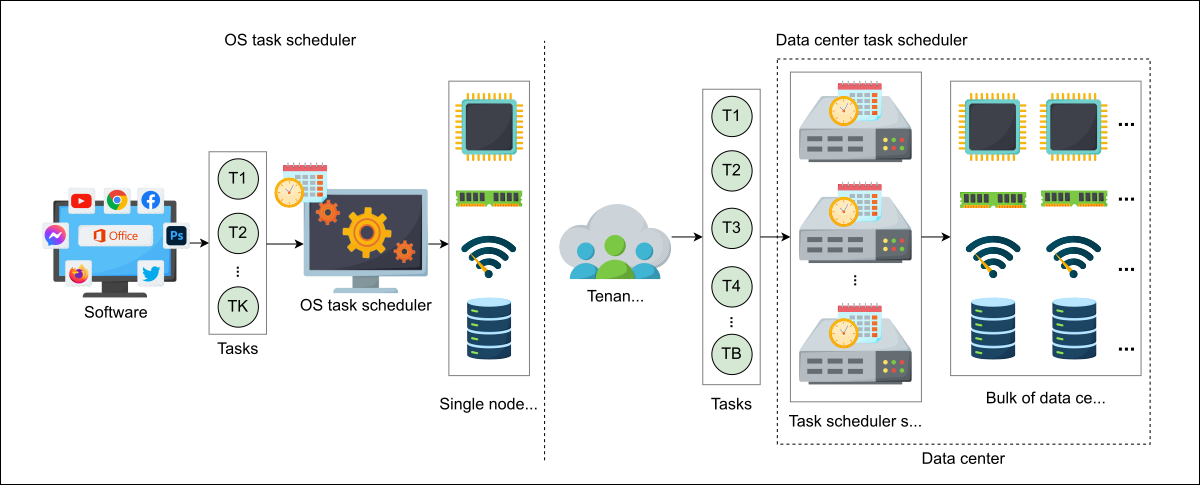
\includegraphics[width=0.5\textwidth]{Images/chapter_23/section_6152021643624448/5296016499015680.png}
 \caption{An OS-level task scheduler vs. a data center-level task scheduler}
\end{figure}

The OS task scheduler schedules a node's local tasks or processes on that node's computational resources. At the same time, the data center's task scheduler schedules billions of tasks coming from multiple tenants that use the data center's resources.
\\
Our goal is to design a task scheduler similar to the data center-level task scheduler where the following is considered:

\begin{itemize}
\item
\protect\phantomsection\label{KJ0aHKz91HdLGCKWcjSio}
Tasks will come from many different sources, tenants, and sub-systems.
\item
\protect\phantomsection\label{iZcKqS2frAJb8dWp6h5o_}
Many resources will be dispersed in a data center (or maybe across many data centers).
\end{itemize}
\\
The above two requirements make the task scheduling problem challenging. We 'll design a distributed task scheduler that can handle all these tasks by making it scalable, reliable, and fault-tolerant.

\subsection{How will we design a task scheduling system?}\label{nZGpv5V819trY277qL4I3}
\\
We have divided the design of the task scheduler into four lessons:

\begin{enumerate}
\item
\protect\phantomsection\label{yWRMPvzCpgSgAU0Sb2OHI}
\href{https://www.educative.io/courses/grokking-the-system-design-interview/requirements-of-a-distributed-task-schedulers-design}{\textbf{Requirements:}} We'll identify the functional and non-functional requirements of a task scheduling system in this lesson.
\item
\protect\phantomsection\label{_6DgH5CcJfYAYDZxUnRiS}
\href{https://www.educative.io/courses/grokking-the-system-design-interview/design-of-a-distributed-task-scheduler}{\textbf{Design:}} This lesson will discuss the system design of our task scheduling system and explores the components of the system and database schema.
\item
\protect\phantomsection\label{MbiY3E9N1JJsTuwiEVg2X}
\href{https://www.educative.io/courses/grokking-the-system-design-interview/design-considerations-of-a-distributed-task-scheduler}{\textbf{Design considerations:}} In this lesson, we'll highlight some design factors, such as task prioritization, resource optimization, and so on.
\item
\protect\phantomsection\label{5kbTJmOu8PGApDd7SzzcK}
\href{https://www.educative.io/courses/grokking-the-system-design-interview/evaluation-of-a-distributed-task-schedulers-design}{\textbf{Evaluation:}} We'll evaluate our design of task scheduler based on our requirements.
\end{enumerate}
\\
Let's start by understanding the requirements of a task scheduling system.

% End of section content